\subsection{MIMO SIC}
For system beyond LTE-Advanced in the future, successive
interference canceller (SIC) in the cellular multiple-input
multiple-output (MIMO) is an important issue.

We consider investigation of NOMA with SIC in the cellular MIMO system.
The idea is to implement SIC to signals within
a single beam controlled by the beamforming (precoding) matrix.
In \cite{Non-orthogonal_Access_with_Random_Beamforming_and_Intra-beam_SIC_for_Cellular_MIMO_Downlink},
the authors propose intra-beam superposition coding of a multiuser signal at
the transmitter and the spatial filtering of inter-beam
interference followed by the intra-beam SIC at the user terminal
receiver. The intra-beam SIC cancels out the inter-user
interference within a beam.
According to \cite{Non-orthogonal_Access_with_Random_Beamforming_and_Intra-beam_SIC_for_Cellular_MIMO_Downlink},
the channel after the spatial filtering is a degraded SISO
channel, and the equivalent normalized channel gain of user
can be formulated as follows:

\begin{equation}
\label{eq:gain_mimo_mmse_rcvr}
\begin{split}
&g_{u,f,b}= \\
&\frac{|\mathbf{v}^H_{u,f,b} \mathbf{H}_{u,f} \mathbf{m}_{f,b}|^2}{\underset{b'\in B, b'\neq b}{\sum} P_{b'}|\mathbf{v}^H_{u,f,b} \mathbf{H}_{u,f} \mathbf{m}_{f,b'}|^2 + \mathbf{v}^{H}_{u,f,b} E[\mathbf{w}_{u,f} \mathbf{w}^{H}_{u,f}] \mathbf{v}_{u,f,b}}
\end{split}
\end{equation}

In equation~\ref{eq:gain_mimo_mmse_rcvr}, 
$\mathbf{v}_{u,f,b}$ denotes the spacial filter vector, in \cite{Non-orthogonal_Access_with_Random_Beamforming_and_Intra-beam_SIC_for_Cellular_MIMO_Downlink},
it is is calculated based on the minimum mean squared error
(MMSE) criteria.
$\mathbf{H}_{u,f}$ denotes the N $\times$ M-dimensional channel matrix between
the base station and user $u$ at frequency block $f$.
$\mathbf{m}_{f,b}$ denotes the transmitter beamforming vector.
$\mathbf{w}_{u,f}$ denotes the receiver noise plus inter-cell interference
vector at frequency block $f$,
and $P_{b}$ is the transmission power of beam $b$.
Therefore, we can apply intra-beam SIC to received signal in the
same way by equation~\ref{eq_sic_shannon}.


%\subsection{Analysis starting from modulation/PER}
%\label{sec_phy_modulation}

In practice, it might not be possible to achieve perfect interference cancellation.
%Without considering partial interference cancellation and modulation, (\ref{eq_sic_shannon}) is too optimistic to evaluate the performance of NOMA with SIC. 
The authors in~\cite{cite_bell1} have show simulation results for SIC with respect to modulation schemes and SNR difference as given in Fig.~\ref{fig_NOMA_modulation}. All points enclosed in the upper right area of each curve are in the desired operating region with $\text{PER} \leq 10^{-2}.$  
Table~\ref{tb_NOMA_modulation} further shows the relationship between modulation and SNR for three marked points in the figure. We can find that the simulation result does not strictly follow (\ref{eq_sic_shannon}). For example, if the SNR of U1 becomes 8 times (i.e. 9 dB) larger, the modulation of U1 can upgrade from QPSK to 16QAM, which has only 2 times larger capacity. 
%
Fig.~\ref{fig_NOMA_modulation} motivates our further investigation on the practical performance of SIC for MAC layer design.
%Therefore, (\ref{eq_sic_shannon}) should be modified and we will analyze how to construct SNR-modulation model and equation in the future works.


\begin{figure}[t]
\begin{center}
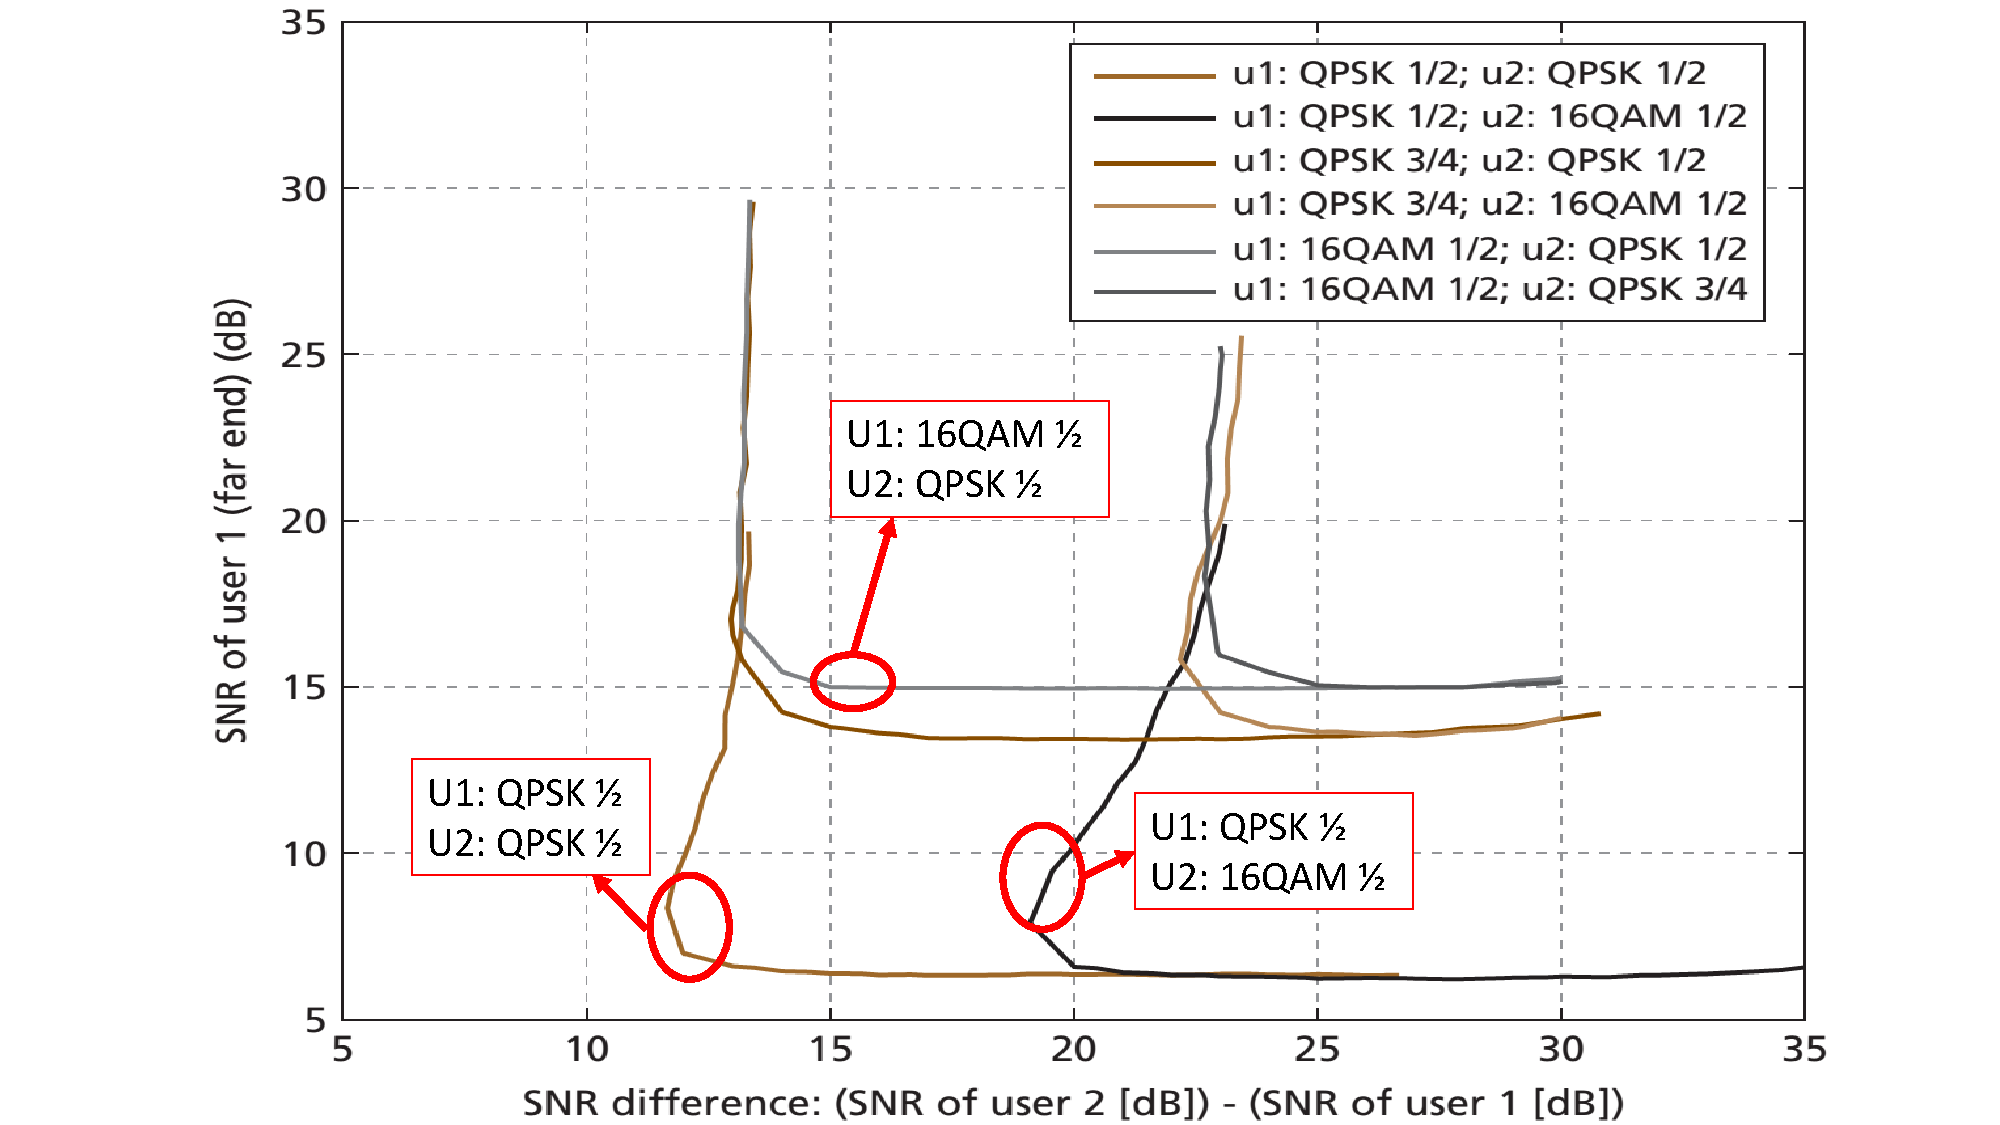
\includegraphics[width=1\columnwidth ,angle=0]{figure/NOMA_modulation}
\caption{Modulation and PER vs. SNR difference}
\label{fig_NOMA_modulation}
\end{center}
\end{figure}
%

\begin{table}[t]
\caption{Modulation curve in Fig.~\ref{fig_NOMA_modulation}}
    \begin{tabular}{| l | l | l | l |}
    \hline
    U1 Modulation & U2 Modulation & SNR of U1 & SNR Diff \\ \hline
    QPSK 1/2       & QPSK 1/2       & 6-15           & 12-20                  \\ \hline
    QPSK 1/2       & 16QAM 1/2     & 6-15           &  $\geq$ 20                     \\ \hline
    16QAM 1/2     & QPSK 1/2       & $\geq$15            & 12-20                   \\ \hline
    \end{tabular}
\label{tb_NOMA_modulation}
\end{table}